%% Los cap'itulos inician con \chapter{T'itulo}, estos aparecen numerados y
%% se incluyen en el 'indice general.
%%
%% Recuerda que aqu'i ya puedes escribir acentos como: 'a, 'e, 'i, etc.
%% La letra n con tilde es: 'n.

\chapter{Soluci\'on Te\'orico-Conceptual-Computacional}

El presente cap\'itulo se enfocar\'a en el marco te\'orico-computacional de la propuesta de soluci\'on, abordando las acciones que pueden realizar los usuarios de OLS y la estructura de la aplicaci\'on, as\'i como la arquitectura y patr\'on de visualizaci\'on empleado. Se explicar\'an, adem\'as, las modificaciones realizadas sobre el c\'odigo fuente del servidor, dando a conocer, finalmente, algunos detalles de implementaci\'on de las nuevas herramientas creadas.

\section{Diagrama de casos de uso en Open Latino Server}
Las funcionalidades de OLS son consumidas por usuarios y aplicaciones cliente. Un usuario representa al humano que accede a la interfaz visual y puede hacer determinados cambios como agregar capas, editar tem\'aticos, crear workspaces, etc\'etera. Un cliente constituye una aplicaci\'on registrada para usar los servicios del servidor de mapas\footnote{Los servicios son los tipos de pedidos que se pueden hacer en OLS, por ejemplo: GetMap, GetCapabilities, entre otros}.


\subsection{Usuarios}
En la aplicaci\'on existen dos roles de usuario: Usuario Regular y Admin. Un Usuario Regular es un usuario que se registra en el sistema, y luego puede ingresar mediante nombre de usuario y contrase\~na, para tener acceso a algunas de las funcionalidades de la aplicaci\'on. Admin es un administrador del sistema, tiene permisos para realizar operaciones CRUD\footnote{acr\'onimo de ¨Crear, Leer, Actualizar y Borrar¨ (del original en ingl\'es: Create, Read, Update and Delete), que se usa para referirse a las funciones b\'asicas en bases de datos o a la capa de persistencia en un software.} sobre las entidades para configurar el servidor. La figura \ref{casos1} representa un diagrama de casos de uso\footnote{Permiten visualizar las interacciones que podr\'ia tener un usuario o un cliente con un sistema.} de las funcionalidades generales que tienen los usuarios en OLS.

Un usuario regular puede realizar las siguientes acciones:

$\bullet$ Registrarse en el sistema.

$\bullet$ Iniciar sesi\'on mendiante nombre de usuario y contrase\~na.

$\bullet$ Registrar sus aplicaciones cliente y crear, editar o eliminar Workspaces para las mismas.



\begin{wrapfigure}{l}{0.5\textwidth} 
\vspace{-20pt} 
\begin{center} 
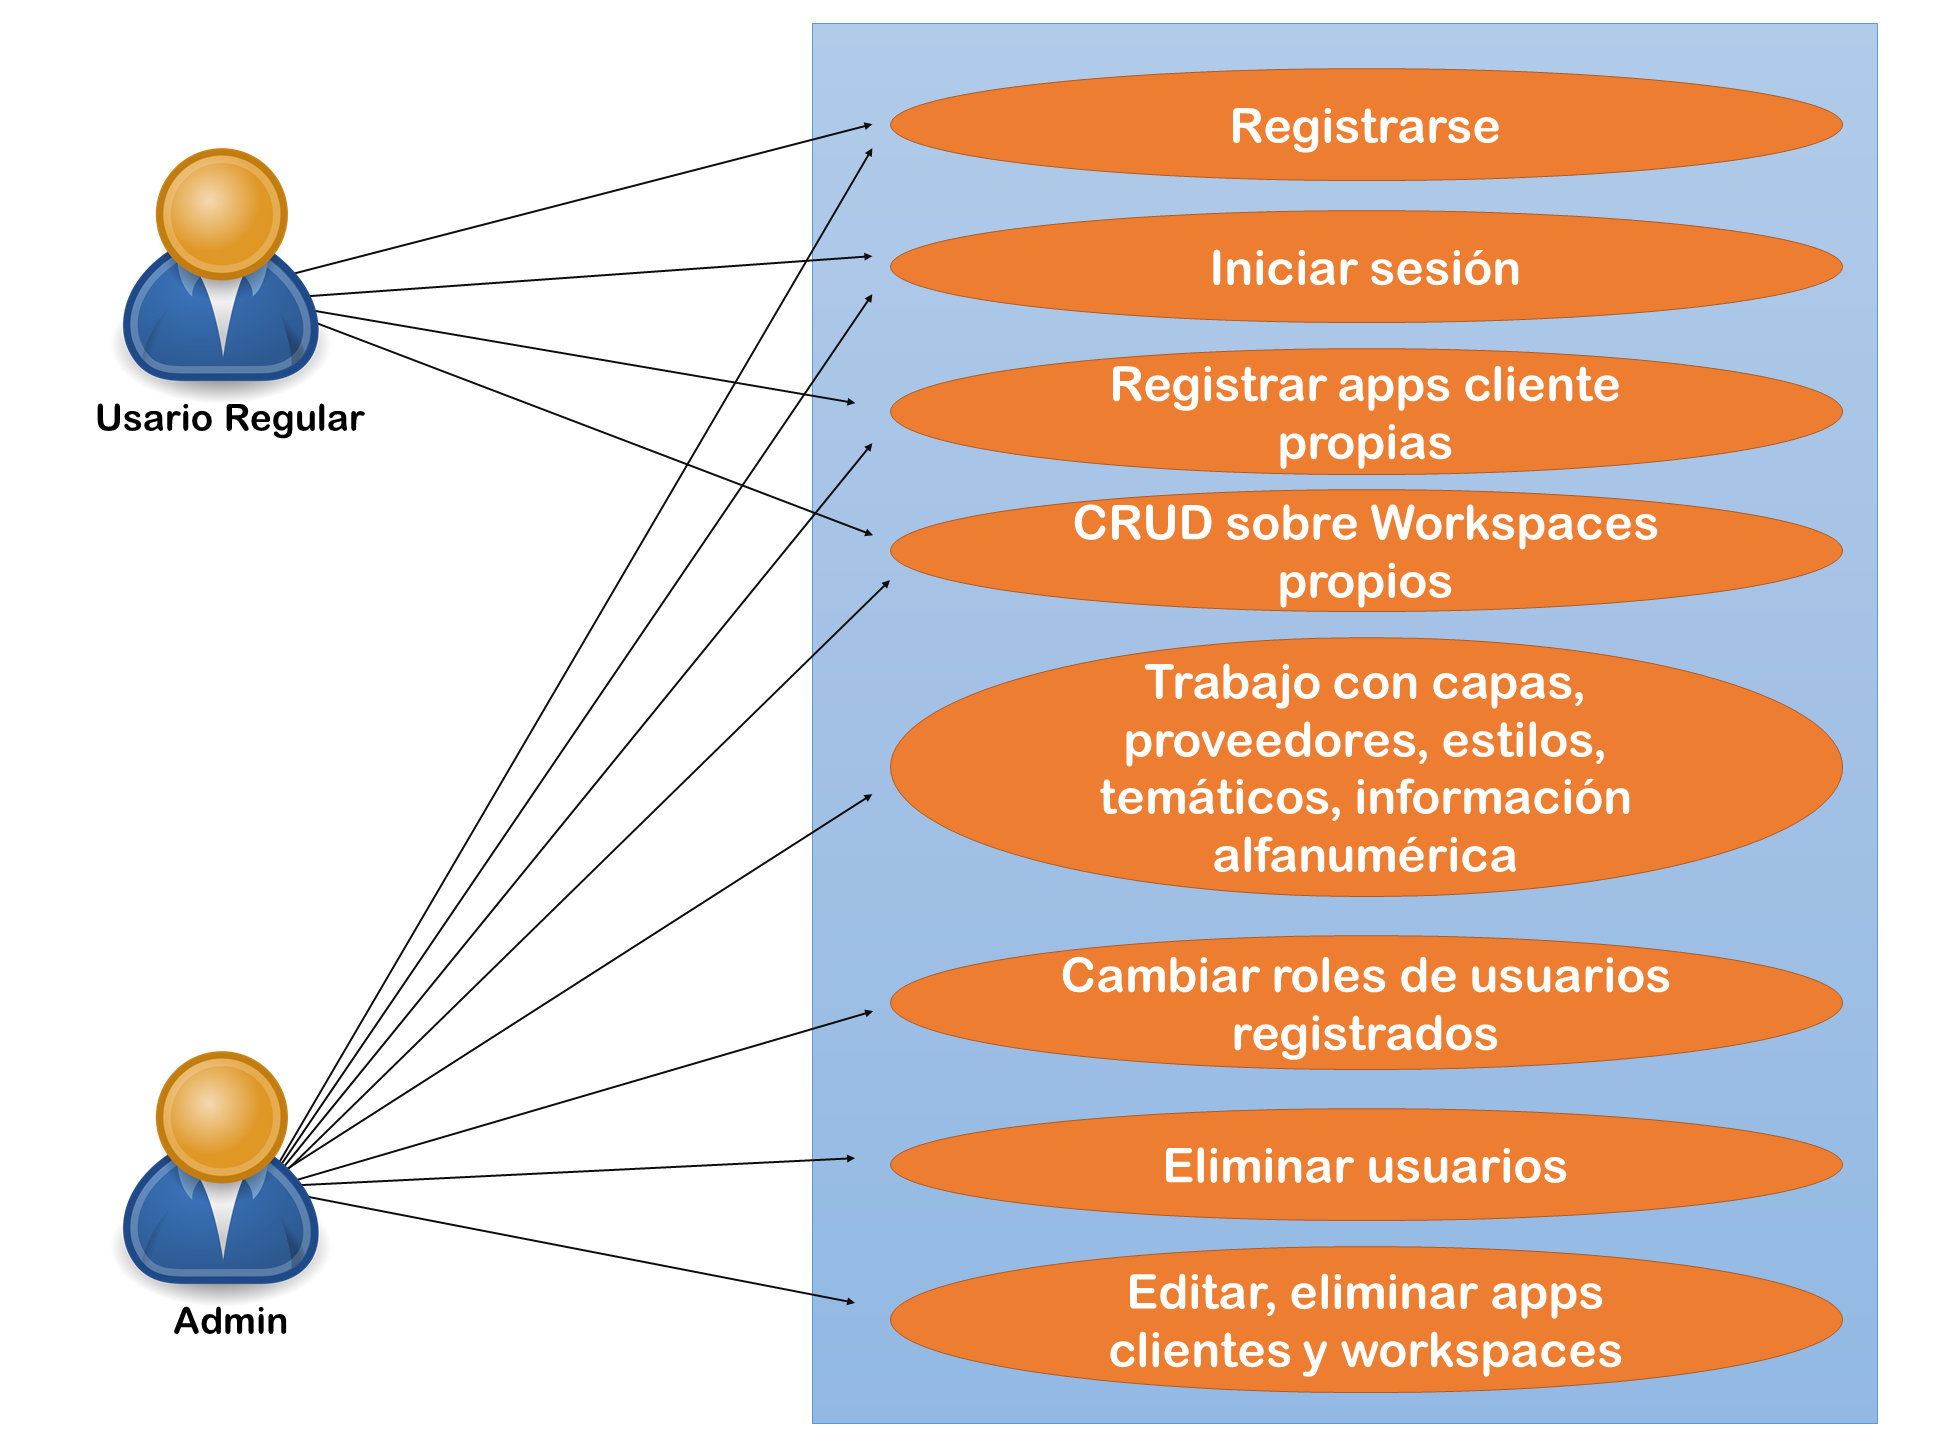
\includegraphics[width=0.52\textwidth]{images/casosdeUsousuario.png} 
\end{center} \vspace{-20pt} \caption{Diagrama de casos de uso de los usuarios en OLS.} \label{casos1}\vspace{-10pt} 
\end{wrapfigure}

Un administrador, adem\'as de realizar todas las acciones de un usuario regular, tambi\'en tiene acceso a las siguientes funcionalidades:

$\bullet$ Crear, editar, eliminar capas, proveedores de datos, estilos, tem\'aticos e informaci\'on alfanum\'erica.

$\bullet$ Cambiar roles de los usuarios registrados en el sistema o eliminarlos totalmente del servidor.

$\bullet$ Tiene acceso a todos los workspaces creados por los usuarios, as\'i como a todas las aplicaciones cliente registradas, pudiendo realizar cambios sobre estos.


\subsection{Aplicaciones cliente}
Los permisos que tienen las aplicaciones cliente para acceder a los servicios de OLS son controlados mediante workspaces. Un Workspace permite restringir las capas y funcionalidades del sistema. Todo cliente que se registra en el nuevo servidor de OpenLatino adquiere acceso a un Workspace llamado \textit{common}. Este espacio de trabajo cuenta con un m\'inimo de funcionalidades y capas para que el cliente pueda usar. Adem\'as, como ya se dijo, el usuario que registr\'o la aplicaci\'on puede crear nuevos Workspaces y as\'i darle acceso a m\'as capas y servicios.

\begin{wrapfigure}{l}{0.5\textwidth} 
\vspace{-20pt} 
\begin{center} 
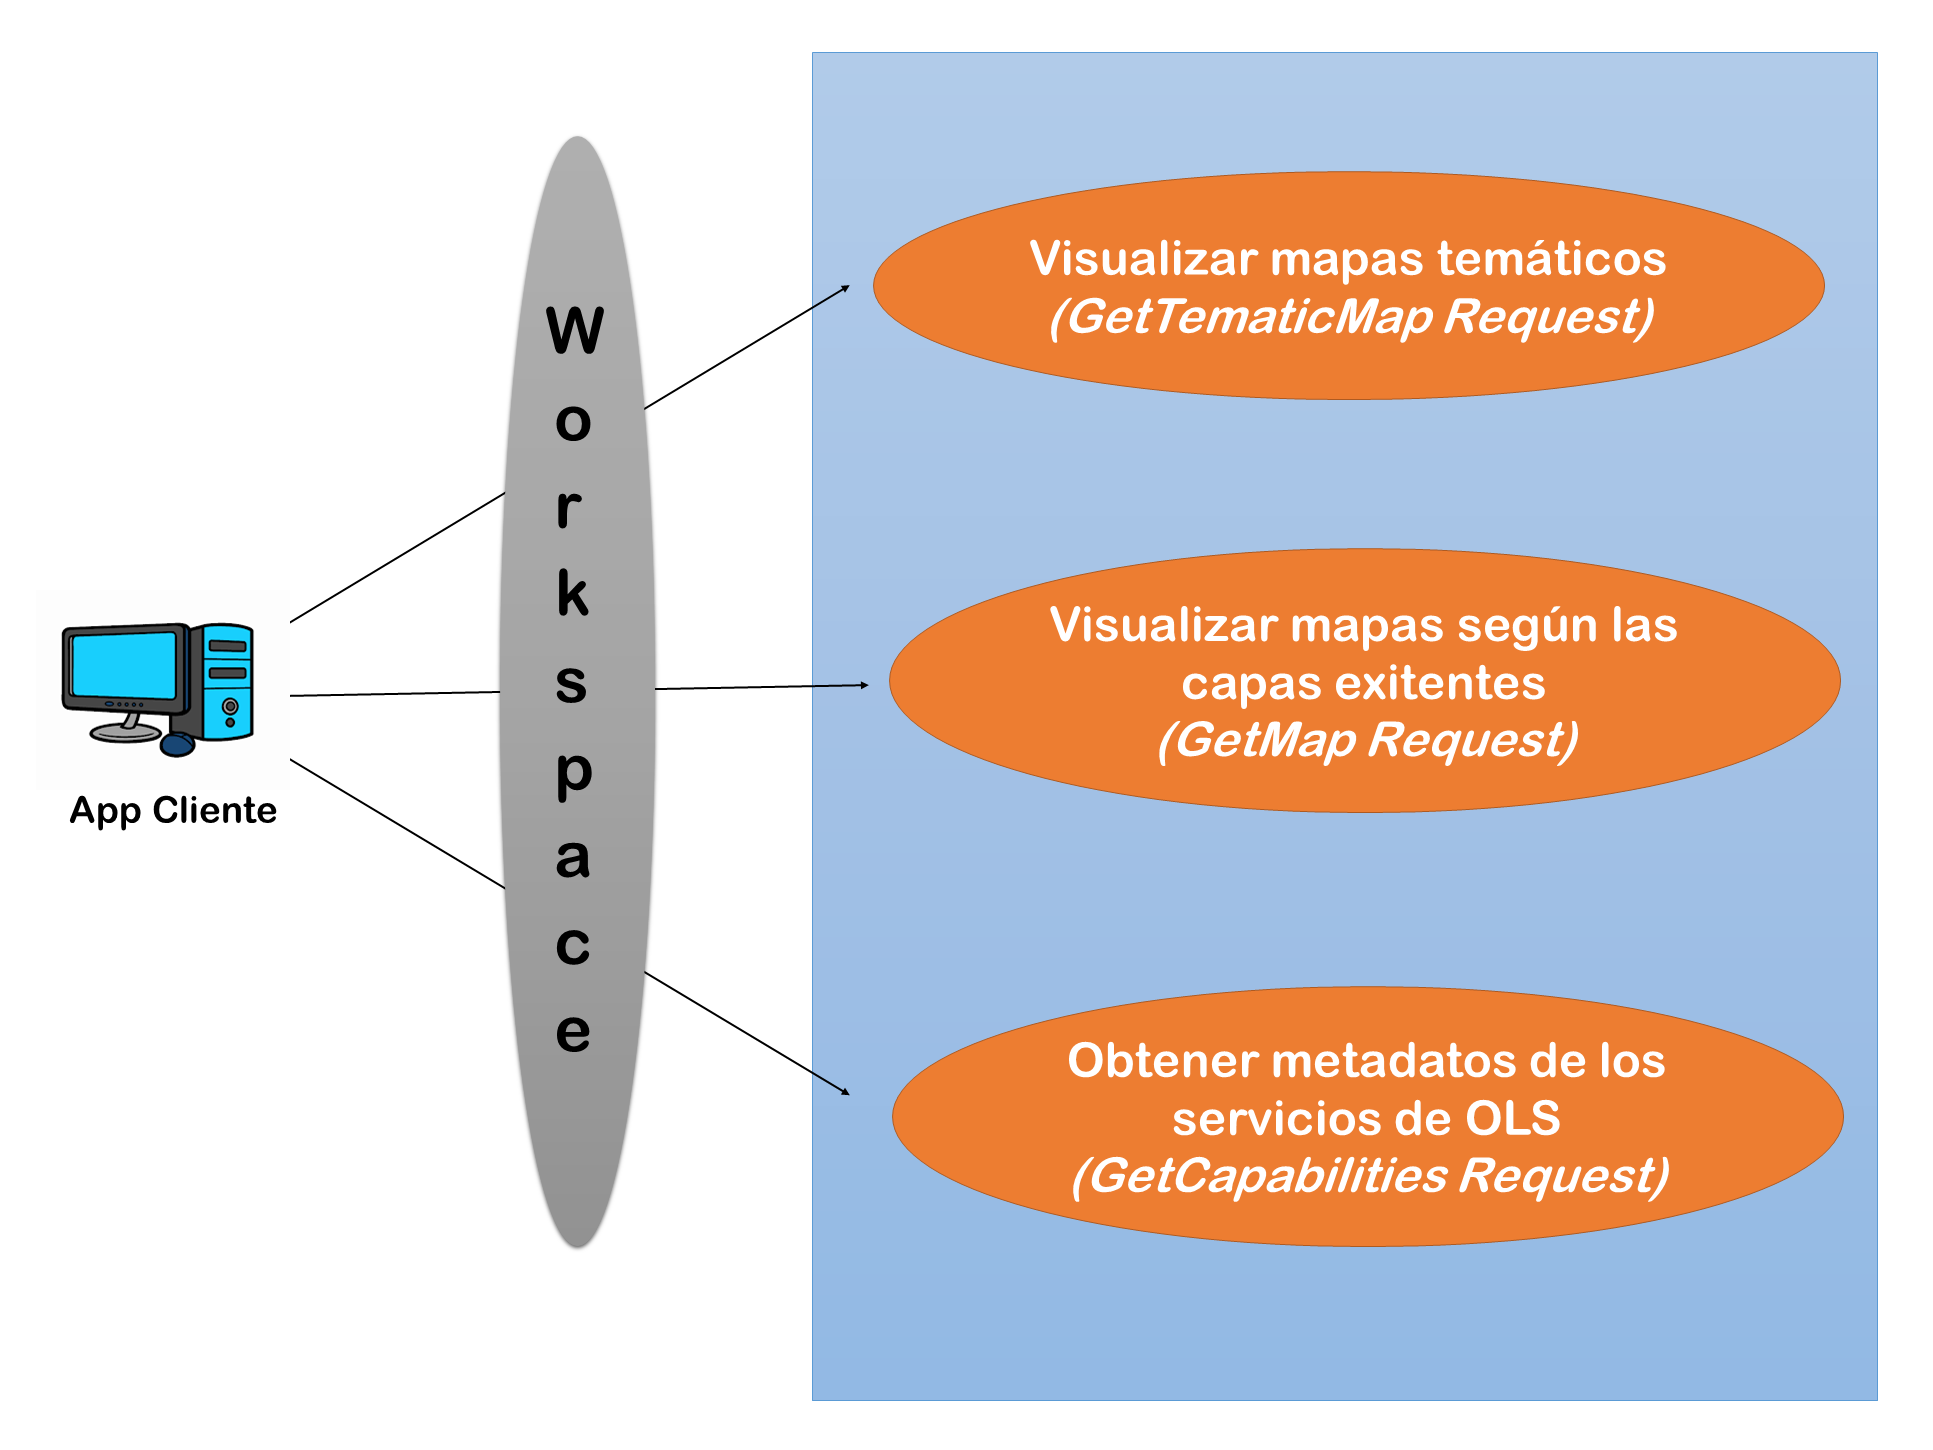
\includegraphics[width=0.52\textwidth]{images/casosdeUsoclient.png} 
\end{center} \vspace{-20pt} \caption{Diagrama de casos de uso de las aplicaciones cliente en OLS.} \label{casos2} \vspace{-10pt} 
\end{wrapfigure}

Cada aplicaci\'on cliente tiene uno o m\'as Workspaces asignados. Como se observa en la figura \ref{casos2}, una aplicaci\'on cliente, con todos los permisos posibles permitidos, tiene acceso a las siguientes funcionalidades:

$\bullet$ Visualizar mapas tem\'aticos definidos en el sistema. (Pedido GetTematicMap)

$\bullet$ Visualizar mapas seg\'un las capas registradas en el servidor. (Pedido GetMap)

$\bullet$ Obtener metadatos de los servicios que ofrece el servidor. (Pedido GetCapabilities)



\section{Modificaci\'on al modelo de datos}
Con el objetivo de crear una herramienta extensible para la creaci\'on de otros tipos de mapas tem\'aticos y, para evitar guardar informaci\'on repetida innecesariamente en la base de datos, se hace necesario la modificaci\'on del modelo de entidades relacionales (MER)\footnote{Herramienta para el modelo de datos, la cual facilita la representaci\'on de entidades de una base de datos.}

\begin{wrapfigure}{l}{0.5\textwidth} 
\vspace{-20pt} 
\begin{center} 
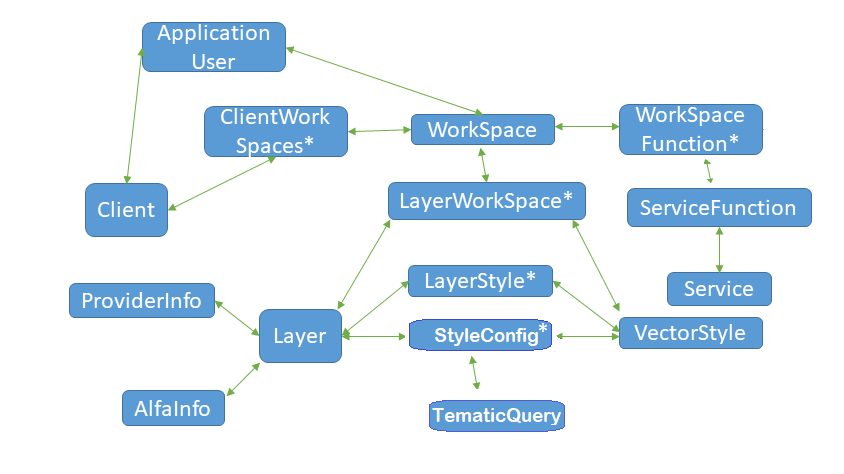
\includegraphics[width=0.53\textwidth]{images/merViejo.png} 
\end{center} \vspace{-20pt} \caption{Modelo de datos de la \'ultima versi\'on de OLS.} \label{merViejo} \vspace{-10pt} 
\end{wrapfigure}

Como se observa en la figura \ref{merViejo}, los tem\'aticos existentes se guardaban en la tabla \textit{TematicQuery}, la cual contiene el nombre del tem\'atico, y una funci\'on serializada que representa la consulta. De esta forma, en la tabla \textit{StyleConfig} se definen los estilos de cada tem\'atico mediante una llave for\'anea al \texttt{Id} de la tabla de tem\'aticos. 

En esta nueva versi\'on de OLS se redefinieron los mapas tem\'aticos para que estos pudieran soportar varias consultas, las cuales, a su vez, puedan soportar varios filtros separados por los operadores AND y OR. La figura \ref{merNuevo} muestra la base de datos modificada, mostrando en color rojo las tablas que sufrieron alguna variaci\'on y en color naranja las tablas que se crearon nuevas. 

\begin{wrapfigure}{l}{0.5\textwidth} 
\vspace{-20pt} 
\begin{center} 
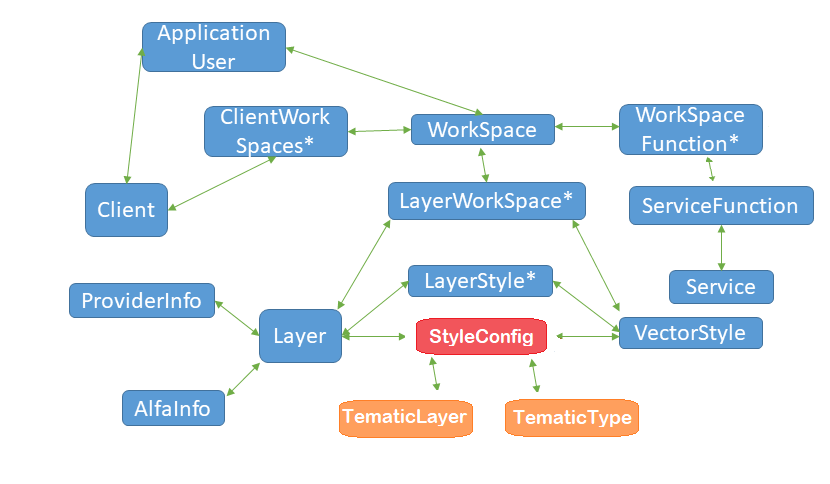
\includegraphics[width=0.53\textwidth]{images/merNuevo.png} 
\end{center} \vspace{-20pt} \caption{Modelo de datos modificado.} \label{merNuevo} \vspace{-10pt} 
\end{wrapfigure}

La tabla \textit{TematicQuery} se elimina, diviendo su contenido en dos nuevas tablas, contendiendo estas, adem\'as, informaci\'on acerca del tipo de tem\'atico.

Se a\~nadi\'o la tabla \textit{TematicLayers}, que representa el concepto de mapa tem\'atico, est\'a conformada por los campos \texttt{Name}, de tipo string y que representa su nombre, e \texttt{Id} que es su identificador de tipo num\'erico. Esta tabla tiene una relaci\'on de uno a muchos con \textit{StyleConfig}, ya que un tem\'atico tiene una o varias configuraciones de estilo, una para cada consulta. Tambi\'en, se cre\'o la tabla \textit{TematicTypes} la cual contiene la informaci\'on de los tem\'aticos, sus filtros, y el tipo de tem\'atico que representa. Esta relacionada con la tabla \textit{StyleConfig} en una relaci\'on de uno a muchos.

Como resultado de la incorporaci\'on de nuevas tablas relacionadas con \textit{StyleConfig}, esta tabla se modific\'o, conteniendo en esta nueva versi\'on la capa, el estilo, y el filtro asociado a un tem\'atico espec\'ifico, como llaves for\'aneas de las respectivas tablas.


\section{Arquitectura de software}
La arquitectura de software es el conjunto de estructuras necesarias para dar sentido a un sistema, lo cual abarca los elementos del software, las relaciones entre ellos y las propiedades de ambos. La arquitectura en capas es una de las m\'as utilizadas, esta se enfoca en la distribuci\'on de roles y responsabilidades de forma jer\'arquica dando una forma muy efectiva de separaci\'on de responsabilidades. El rol indica el modo y tipo de interacci\'on con otras capas, y la responsabilidad indica la funcionalidad que est\'a siendo desarrollada. \cite{architecture2}

\begin{wrapfigure}{l}{0.5\textwidth} 
\vspace{-20pt} 
\begin{center} 
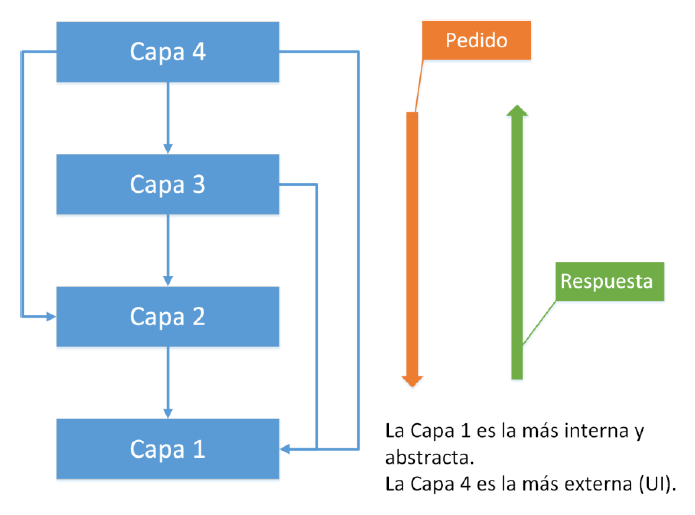
\includegraphics[width=0.52\textwidth]{images/arquitecturaFlexible.png} 
\end{center} \vspace{-20pt} \caption{Ejemplo de Arquitectura de capas con 4 capas en su forma flexible.} \label{flexible} \vspace{-10pt} 
\end{wrapfigure}

En una arquitectura de capas, todas las capas se colocan de forma horizontal, donde una capa solo puede depender otra que est\'e por debajo de ella, nunca por encima. En una forma estricta de la arquitectura, solo se puede acceder a la capa que est\'a exactamente debajo. Si se usa un acercamiento m\'as flexible, como se puede observar en la Figura \ref{flexible}, una capa puede acceder a todas las capas por debajo de ella. \cite{architecture}

La arquitectura de capas divide la aplicaci\'on con la intenci\'on de que cada una tenga un rol muy definido, no define la cantidad de capas que debe tener la aplicaci\'on y aplica el principio de separaci\'on de preocupaciones. La ventaja principal de este estilo es que el desarrollo se puede llevar a cabo en varios niveles y, en caso de tener que hacer alg\'un cambio, solo se realiza en el nivel que le corresponda.

\subsection{Modificaciones a la arquitectura de OLS}
OpenLatino Server implementa \textit{Clean Architecture}\footnote{Arquitectura limpia en espa\~nol. Presentada por Robert C. Martin (Uncle Bob) en su blog, el 13 de agosto de 2012 \cite{cleanArchitecture}}, la cual es una arquitectura por capas.  En la figura \ref{cleanArchitecture} se muestra la Arquitectura de software \textit{Clean Architecture} implementada en OLS. Se puede observar la separaci\'on de las capas y la dependencia que existe entre ellas.

\begin{wrapfigure}{l}{0.5\textwidth} 
\vspace{-20pt} 
\begin{center} 
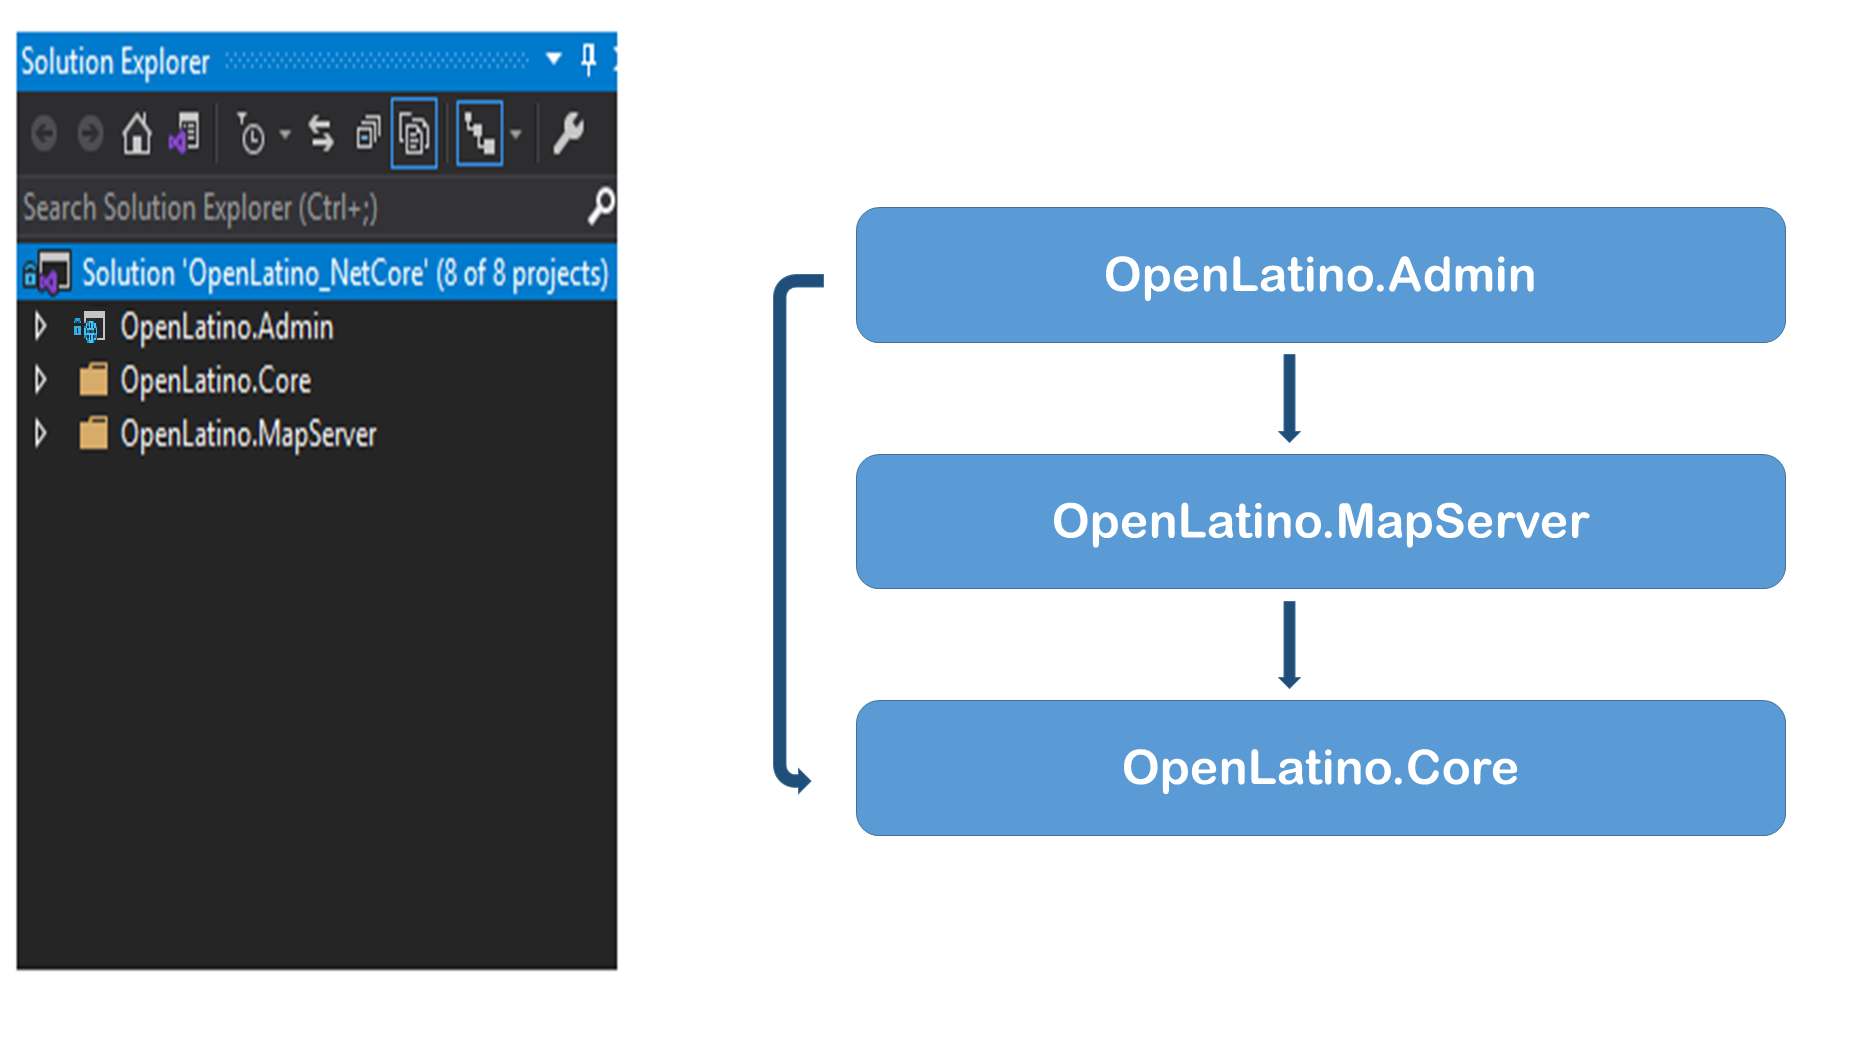
\includegraphics[width=0.53\textwidth]{images/cleanArchitecture.png} 
\end{center} \vspace{-20pt} \caption{Arquitectura de software \textit{Clean Architecture} implementada en OLS en su \'ultima versi\'on.} \label{cleanArchitecture} \vspace{-10pt} 
\end{wrapfigure}

En la \'ultima versi\'on, OLS presenta tres capas:

$\bullet$ \textbf{OpenLatino.Core}. Es la capa base. No tiene dependencias externas. Posee las entidades y la declaraci'on de las interfaces.

$\bullet$ \textbf{OpenLatino.MapServer.} Depende de la capa OpenLatino.Core. Se encarga de procesar los pedidos de las aplicaciones cliente y devolver un response. Posee la implementaci\'on de las funciones WMS.

$\bullet$ \textbf{OpenLatino.Admin}. Depende de las capas anteriores, posee la implementaci\'on de los controladores encargados de recibir las peticiones de las aplicaciones cliente.

En la nueva versi\'on de OLS, con la implementaci\'on de la interfaz visual de configuraci\'on en Angular, se hizo necesario modificar la arquitectura, manteniendo los principios de \textit{Clean Architecture}, garantizando la extensibilidad, seguridad y buenas pr\'acticas del servidor. La nueva arquitectura de OLS se muestra en la figura \ref{cleanArchitectureNew}.

Se elimin\'o la capa m\'as externa de la arquitectura de OLS y, en su lugar, se implementaron tres nuevas capas:

$\bullet$ \textbf{OpenLatino.Admin.Infraestructure}. Consiste en una capa de abstracci\'on entre la entre la capa de entidades de dominio y la capa de l\'ogica de negocio. Implementa el patr\'on Repositorio \footnote{Patr\'on de dise\~no que a\'isla la capa de datos del resto de la aplicaci\'on.}, que consulta la fuente de datos, los asigna a una entidad y realiza cambios en dicha entidad a la fuente de datos.

\begin{wrapfigure}{l}{0.5\textwidth}
\vspace{-20pt}
\begin{center}
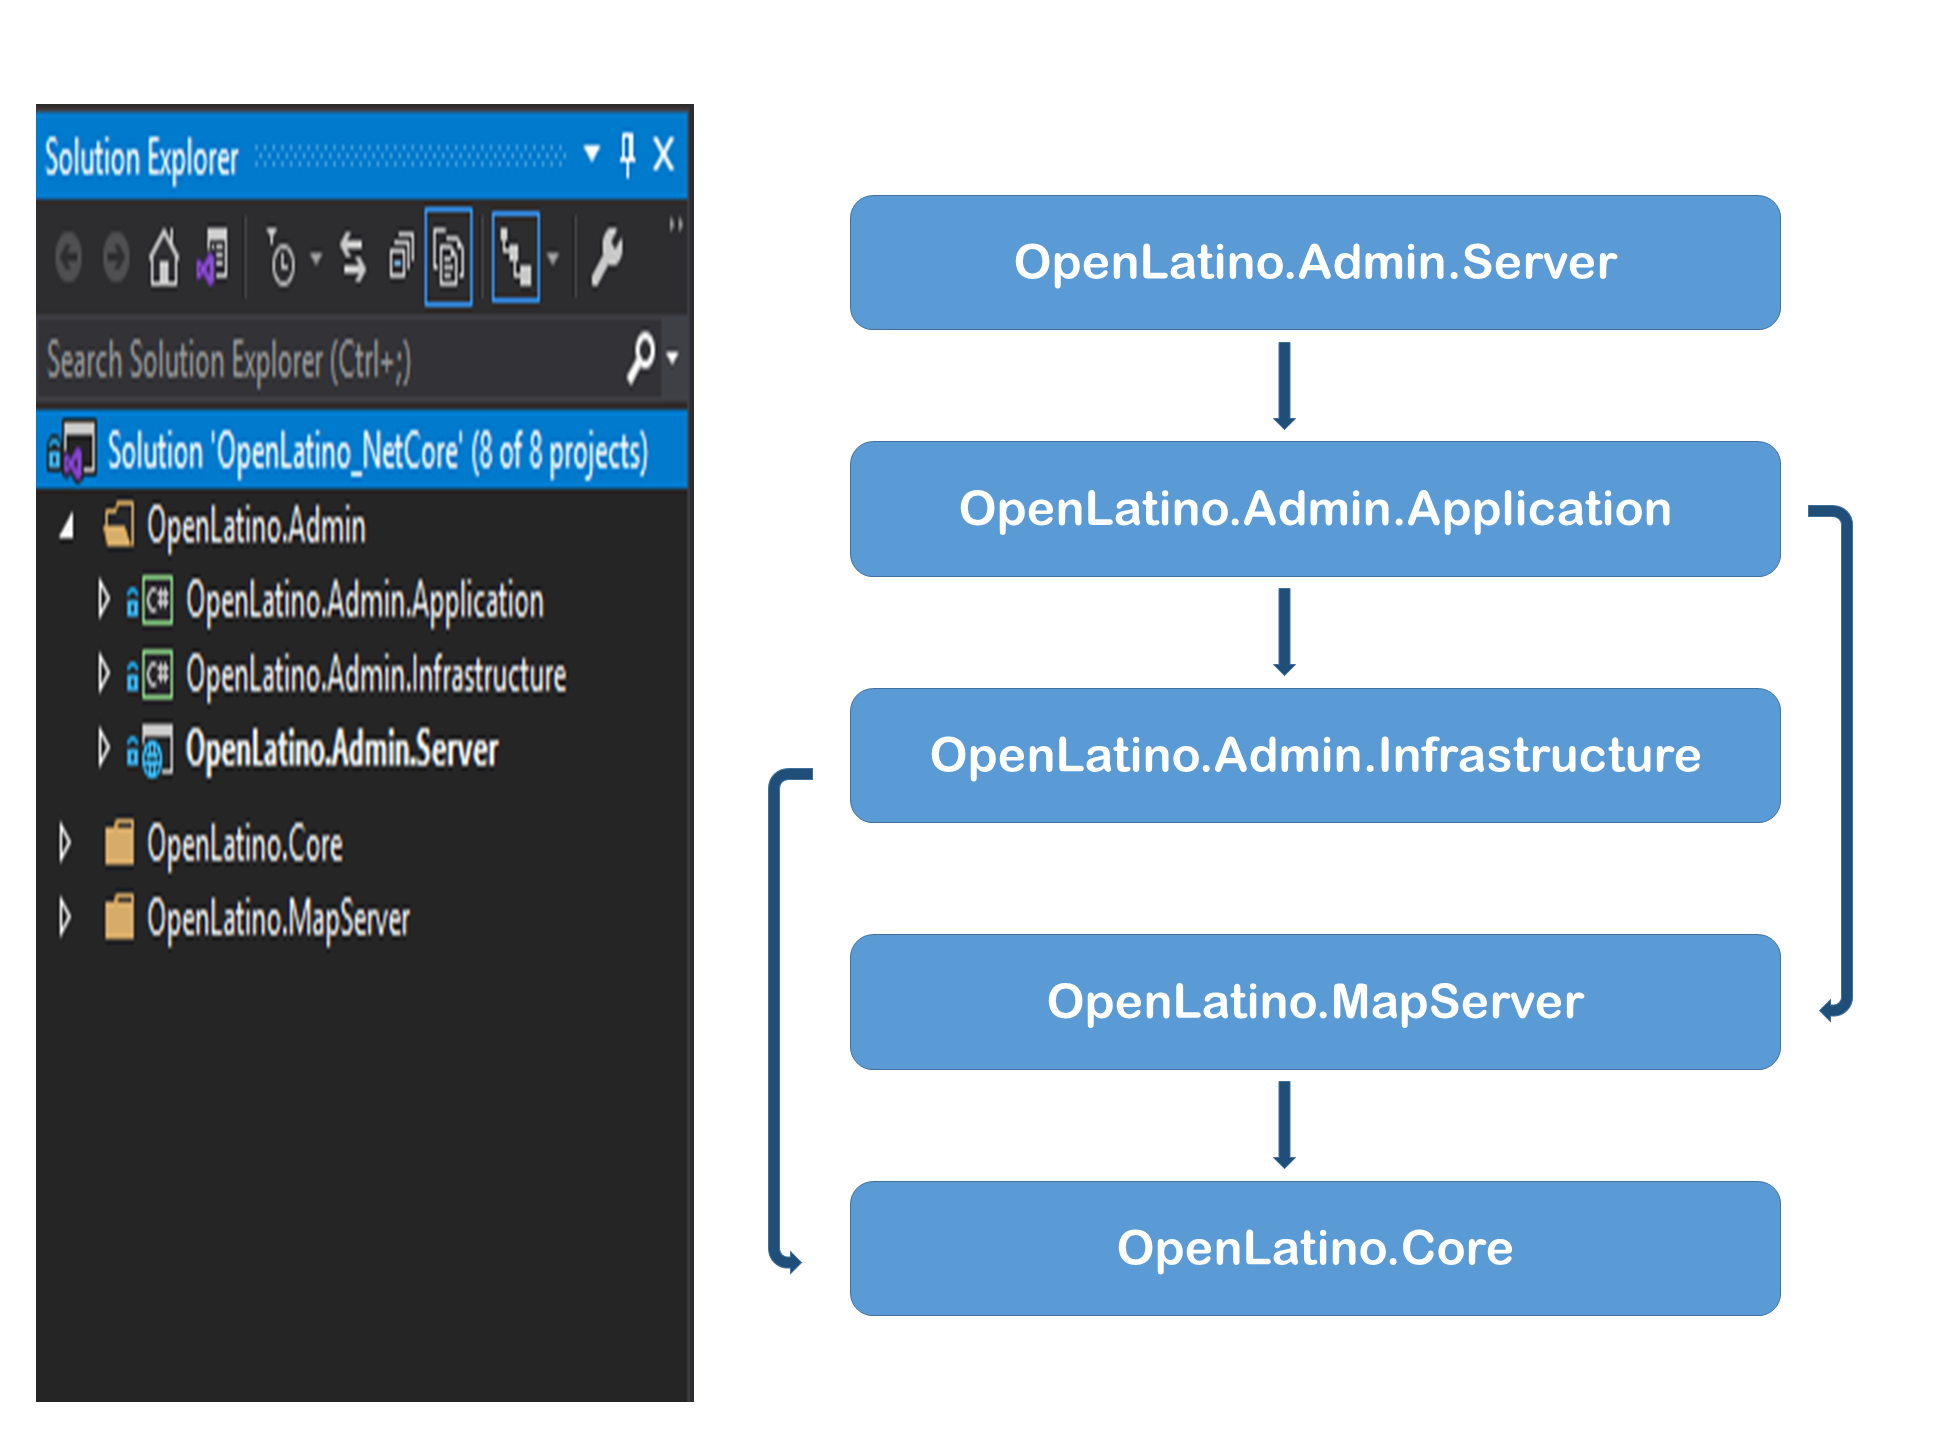
\includegraphics[width=0.52\textwidth]{images/cleanArchitectureNew.png} 
\end{center} \vspace{-20pt} \caption{Arquitectura de software \textit{Clean Architecture} de OLS modificada.}  \label{cleanArchitectureNew} \vspace{-10pt} 
\end{wrapfigure}

$\bullet$ \textbf{OpenLatino.Admin.Application}. Esta capa contiene interfaces que se utilizan para comunicarse entre la capa OpenLatino.Admin.Server y la capa de repositorio. Contiene los servicios asociados a una entidad espec\'ifica, ya sean proveedores, tem\'aticos, estilos, etc.

$\bullet$ \textbf{OpenLatino.Admin.Server} Es la capa m\'as externa de la aplicaci\'on, contiene los controladores que reciben los pedidos de las aplicaciones clientes y de los usuarios de la interfaz visual de configuraci\'on. En esta capa se realiza, adem\'as, la verificaci\'on de seguridad, que valida la identidad de los usuarios y clientes que realizan los pedidos.


\subsection{Arquitectura de la Interfaz Visual de Configuraci\'on.}
Las aplicaciones creadas con Angular se separan en plantillas HTML, clases de componentes en TypeScript, escritas para gestionar dichas plantillas, y los servicios que contienen la l\'ogica para la comunicaci\'on con el servidor. 

Para crear la interfaz visual se generaron templates con HTML, controlando estos con l\'ogica creada en componentes, que ser\'an exportados como clases. As\'i mismo, se agregan los servicios para manejar el flujo de datos de la aplicaci\'on y el servidor OLS. Finalmente, se ''encapsulan'' dichas componentes y servicios en m\'odulos. 

\begin{wrapfigure}{l}{0.5\textwidth}
\vspace{-20pt}
\begin{center}
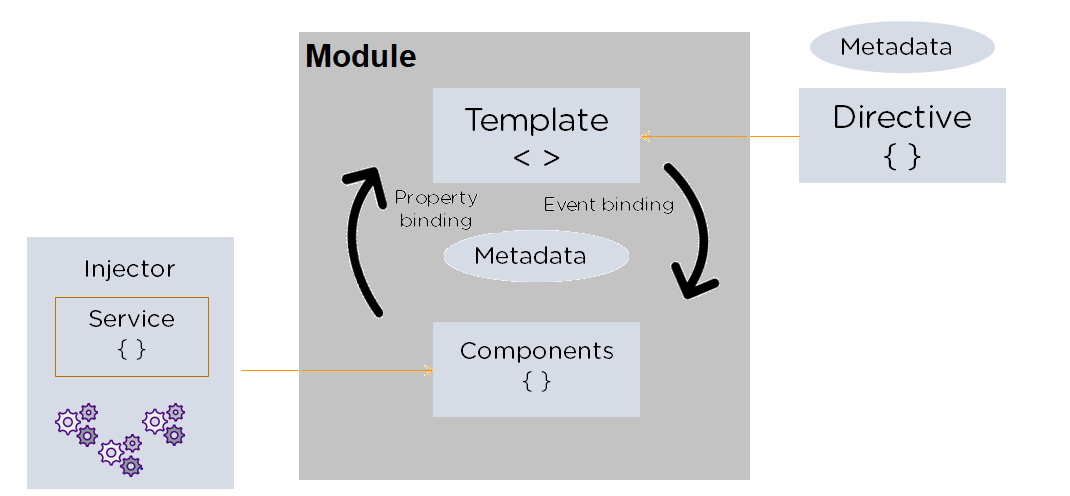
\includegraphics[width=0.52\textwidth]{images/angularArchitecture.png} 
\end{center} \vspace{-20pt} \caption{Arquitectura de software de la interfaz visual.}  \label{arquitecturaAngular} \vspace{-10pt} 
\end{wrapfigure}

La arquitectura de la aplicaci\'on desarrollada se muestra en la figura \ref{arquitecturaAngular}. Con el objetivo de seguir las buenas pr\'acticas de la programaci\'on, la interfaz visual implementa varios m\'odulos cuyas funcionalidades est\'an bien definidas e independientes. Estos gestionan el trabajo con tem\'aticos, estilos, proveedores, informaci\'on alfanum\'erica, auntenticaci\'on, etc\'etera. Cada uno de dichos m\'odulos contiene uno o varios servicios que se encargan de realizar los pedidos al servidor, atendiendo a las peticiones del usuario, y de recibir la respuesta de OLS. Estos servicios son inyectados en las componentes como dependencias.

Las componentes son clases que contienen la plantilla de la vista, y la l\'ogica asociada a esta, de una parte de la interfaz visual. Para gestionar la configuraci\'on de OLS se crearon varias componentes, encargadas de crear nuevos tem\'aticos, editar estilos, registrar usuarios, etc\'etera. En la interfaz visual, las plantillas HTML contienen directivas que le proveen l\'ogica de programaci\'on, las cuales realizan \textit{data binding}, es decir, enlazan la l\'ogica de los datos de la aplicaci\'on con las vistas. Por otro lado, \textit{event binding}, responde a la acci\'on del usuario al interactuar en la aplicaci\'on, actualizando los datos en la l\'ogica.


\section{Detalles de implementaci\'on}
En esta secci\'on se explicar\'an los cambios en el c\'odigo para la creaci\'on del nuevo tipo de mapa tem\'atico de categor\'ias, explicando el proceso para crear nuevos tipos de tem\'aticos. Se abordar\'a, tambi\'en, c\'omo fue implementada la seguridad de la interfaz visual y del servidor, no sin antes abordar en qu\'e consiste el est\'andar de seguridad JWT (JSON Web Token por sus siglas en ingl\'es).

\subsection{Implementaci\'on de mapas tem\'aticos}
Para crear el nuevo tipo de mapa tem\'atico se elimin\'o la entidad \texttt{TematicQuery}, creando en su lugar la nueva entidad \texttt{TematicType} (figura \ref{tematicType}), la cual contiene las propiedas inherentes a todo tipo de tem\'atico: Id, nombre, funci\'on, que constituye los filtros, y los estilos asociados. Se cre\'o, adem\'as, la entidad \texttt{TematicLayer} que contiene el nombre y el Id del tem\'atico.

\begin{wrapfigure}{l}{0.5\textwidth}
\vspace{-20pt}
\begin{center}
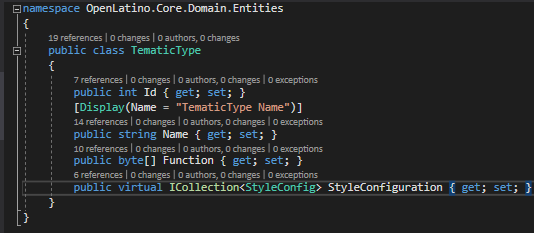
\includegraphics[width=0.52\textwidth]{images/tematicType.png} 
\end{center} \vspace{-20pt} \caption{Entidad que representa los tipos de tem\'aticos en OLS.}  \label{tematicType} \vspace{-10pt} 
\end{wrapfigure}

Para crear nuevos tem\'aticos se crea una nueva clase que herede de la nueva entidad \texttt{TematicType} (figura \ref{nuevosTipos}). 

\begin{wrapfigure}{l}{0.5\textwidth}
\vspace{-20pt}
\begin{center}
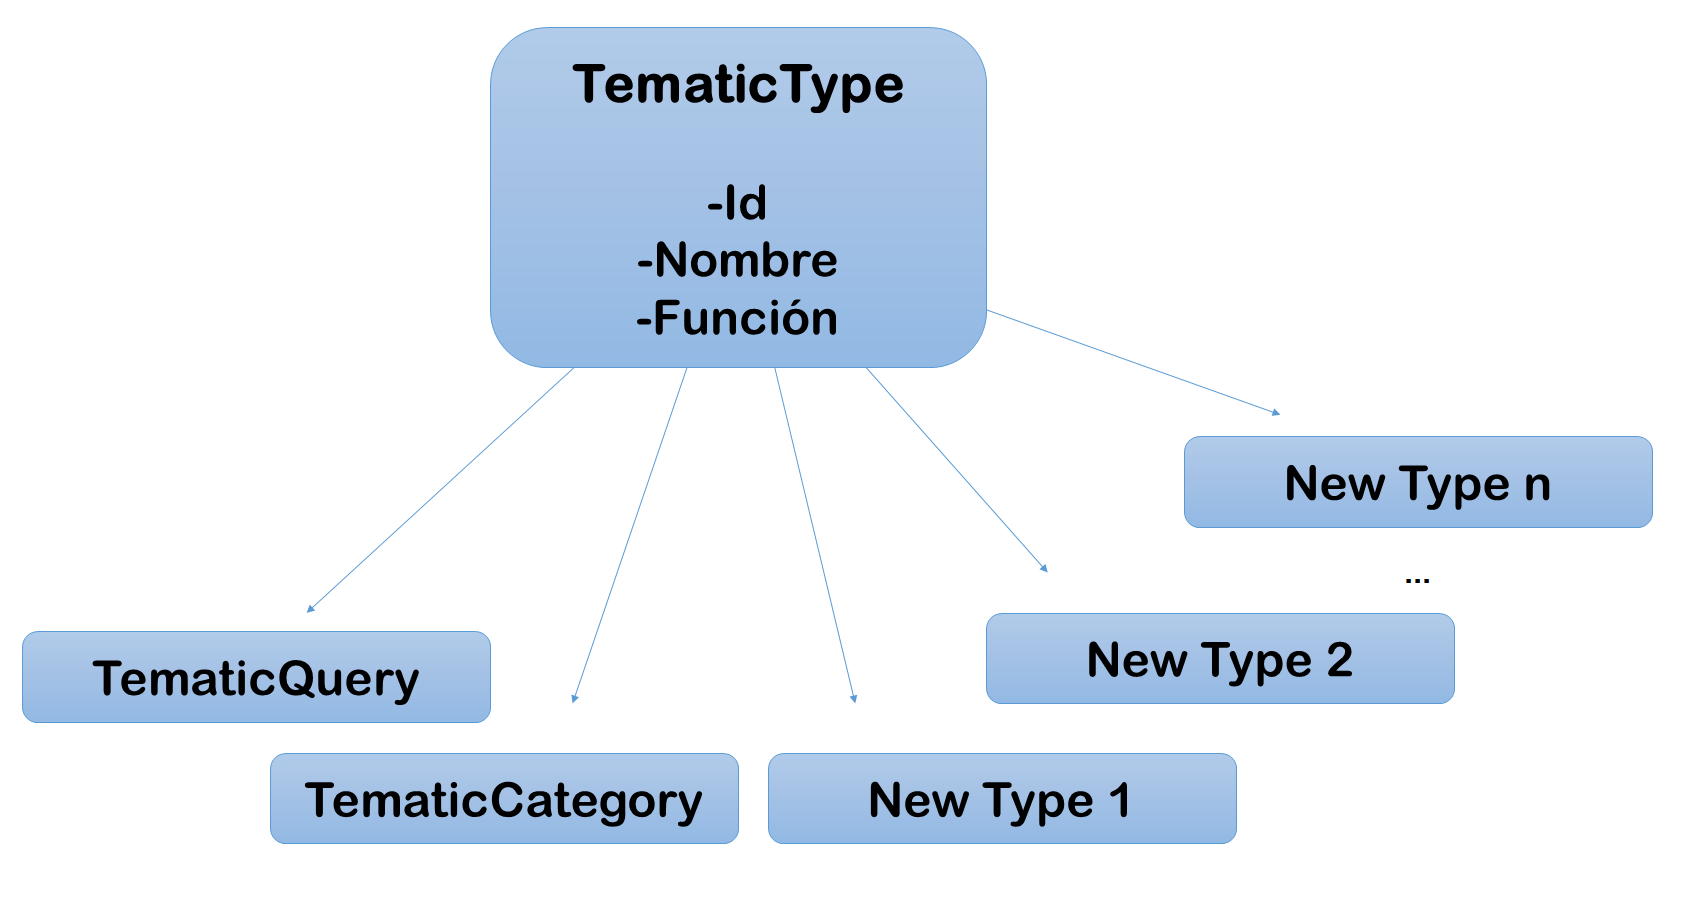
\includegraphics[width=0.52\textwidth]{images/newTematicTypes.png} 
\end{center} \vspace{-20pt} \caption{Estructura para crear nuevos tipos de mapas tem\'aticos.}  \label{nuevosTipos} \vspace{-10pt} 
\end{wrapfigure}

Al heredar de esta clase, autom\'aticamente la clase queda relacionada con la entidad \texttt{StyleConfig}, de esta manera no hay que modificar nada en la estructura existente: se crea la nueva entidad, se agrega alg\'un campo extra que necesite tener y se genera una nueva migraci\'on porque se modifica la base de datos existente al agregar el nuevo tipo.

Se crea, adem\'as, una interfaz \texttt{ITematicLayer Helper}, en sustituci\'on de la interfaz existente, que tiene los m\'etodos que permiten el trabajo con mapas tem\'aticos. El servicio \texttt{TematicLayerService} implementa esta interfaz. 

Para el procesamiento de nuevos tipos de tem\'aticos, se pueden seguir cualquiera de las siguientes v\'ias, dependiendo de lo que se desea implementar:

$\bullet$ \textbf{ITematicLayerHelper} $\rightarrow$ \textbf{TematicLayerService}. Usar el mismo servicio implementado para los tem\'aticos existentes.

$\bullet$ \textbf{ITematicLayerHelper} $\rightarrow$ \textbf{TematicLayerService} $\rightarrow$ \textbf{NewService}. Crear un nuevo servicio que use algunos m\'etodos del servicio existente, redefina otros y cree algunos nuevos.

$\bullet$ \textbf{ITematicLayerHelper} $\rightarrow$ \textbf{NewService}. Crear un nuevo servicio que tenga una implementaci\'on diferente de los m\'etodos actuales.

$\bullet$ \textbf{NewInterfaceHelper} $\rightarrow$ \textbf{NewService}. Crear una nueva interface, y un servicio que la implemente (para mantener la estructura de la aplicaci\'on) debido a que el nuevo tem\'atico usa m\'etodos diferentes a los definidos en la existente.

La opci\'on a escoger var\'ia de acuerdo a las necesidades del programador, dependiendo de las funcionalidades del nuevo tem\'atico a implementar.



\subsection{Seguridad de la interfaz visual y del servidor}
En esta nueva versi\'on de OLS es necesario implementar seguridad a nivel de Usuarios, para controlar las acciones que pueden realizar en la configuraci\'on del servidor desde la interfaz visual, y evitar pedidos de usuarios maliciosos. Igualmente se hace necesario implementar seguridad en los componentes de la interfaz visual, ya que un usuario no autorizado no puede acceder a algunas vistas restringidas en la aplicaci\'on. Para lograr lo anterior se decide implementar Json Web Token (JWT).

Json Web Token (JWT) es un est\'andar para transmitir informaci\'on de forma segura en internet, por medio de archivos en formato JSON\footnote{Tipo de archivo de texto plano con el cual se pueden crear par\'ametros y asignarles un valor}. Este sistema se utiliza en la autenticaci\'on de la interfaz visual, siendo su funci\'on principal la de validar la identidad de quien ingresa a la p\'agina, despu\'es de que ya haya iniciado sesi\'on en el pasado (figura \ref{login}). 

\begin{wrapfigure}{l}{0.5\textwidth}
\vspace{-20pt}
\begin{center}

\includegraphics[width=0.52\textwidth]{images/login.png} 
\end{center} \vspace{-20pt} \caption{Login en OLS desde la interfaz visual.}  \label{login} \vspace{-10pt} 
\end{wrapfigure}

El contenido del token se encuentra firmado digitalmente, por lo que se puede comprobar su veracidad. Gracias a esta certificaci\'on, el servidor web puede aprobar de forma segura todas las peticiones que se hagan desde esa sesi\'on en nombre de ese usuario. Un JWT se divide en tres partes: el \textit{header}, que contiene el tipo de token y la informaci\'on del algoritmo de codificaci\'on\footnote{Usualmente HS256, que genera una firma sim\'etrica, esto quiere decir que el secret/key se usa tanto para el firmado como para la verificaci\'on de la firma.} usado. El \textit{Payload}, que contiene la informaci\'on relativa al usuario, si es admin o usuario regular, cuando inici\'o sesi'on, su Id en el sistema, etc\'etera.

\begin{wrapfigure}{l}{0.5\textwidth}
\vspace{-20pt}
\begin{center}
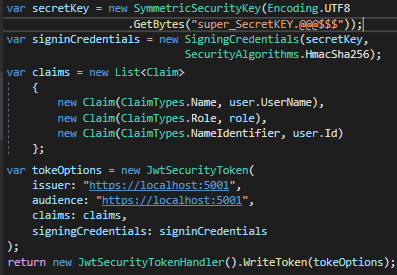
\includegraphics[width=0.52\textwidth]{images/jwtOLS.png} 
\end{center} \vspace{-20pt} \caption{JWT en OLS.}  \label{jwtOLS} \vspace{-10pt} 
\end{wrapfigure}

Finalmente, \textit{Signature} contiene la firma digital del token, creada combinando el header y el payload, basado en una clave secreta que solo el servidor conoce. Los JWT se generan en OLS cuando un usuario inicia sesi\'on en el sistema, la figura \ref{jwtOLS} muestra el fragmento de c\'odigo donde se crea el token y se retorna a la vista. \texttt{JwtSecurityToken} contiene importantes par\'ametros: los dos primeros son para verificar que OLS es el que esta respondiendo los pedidos a la vista, la tercera propiedad contiene informaci\'on acerca del usuario que inici\'o sesi\'on en el sistema; el \'ultimo par\'ametro contiene la firma digital.

A\'un con todas las comprobaciones que se realizan, existe un problema grave de seguridad, ya que un agente externo puede interceptar los pedidos que viajan a OLS desde la interfaz visual y obtener un token que no es suyo, esto implica que puede usarlo para realizar pedidos al servidor como si fuera ese cliente y acceder a informaci\'on confidencial sin ser detectado. 

Para resolver este problema se le establece un tiempo de vida limitado para cada token, es decir, cada uno de los tokens que se les entrega a los clientes ser\'a v\'alido solo por un tiempo prefijado. Este cambio garantiza que, si un token es robado, una vez que se agote su tiempo de vida, no servir\'a. En el caso de OLS, se a\~nade la propiedad \texttt{ expires: DateTime.Now.AddMinutes(30)} al JWT, lo que quiere decir que un usuario se mantendr\'a registrado en el sistema solo por media hora, pasado ese tiempo debe volver a ingresar mediante su contrase\~na.

\begin{wrapfigure}{l}{0.5\textwidth}
\vspace{-20pt}
\begin{center}
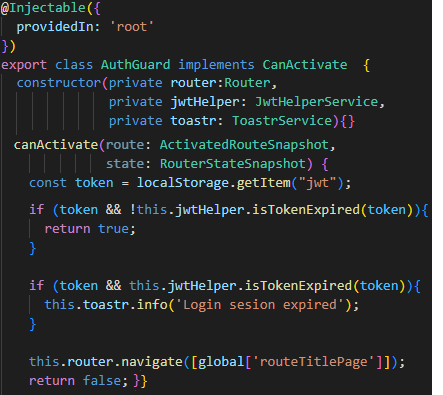
\includegraphics[width=0.52\textwidth]{images/authAngular.png} 
\end{center} \vspace{-20pt} \caption{Seguridad en la interfaz visual.}  \label{auth} \vspace{-10pt} 
\end{wrapfigure}

Del lado del FrontEnd tambi\'en se hacen verificaciones de seguridad, mediante el JWT enviado desde el servidor. Se realizan validaciones, permintiendo a los usuarios acceder a las  vistas de configuraci\'on, seg\'un sus roles. Un usuario que no est\'a logeado no puede acceder a ninguna vista de configuraci\'on, adem\'as, si no es administrador no puede acceder a todas las vistas. En el \texttt{app-routing-module}, mediante la propiedad \texttt{canActivate}, se reciben, por inyecci\'on de dependencia, las clases que verifican, de acuerdo al JWT, si el usuario tiene acceso a la ruta solicitada. En la figura \ref{auth} se muestra la clase encargada de verificar si un usuario esta logeado y si su sesi\'on no ha expirado.

Finalmente, se incluyen los los JWT en los pedidos del FrontEnd a OLS en el header de Autorizaci\'on\footnote{Authorization header, en ingl\'es, contiene las credenciales para autenticar a un usuario en un servidor}.

\begin{wrapfigure}{l}{0.5\textwidth}
\vspace{-20pt}
\begin{center}

\includegraphics[width=0.52\textwidth]{images/request.png} 
\end{center} \vspace{-20pt} \caption{Pedido de la interfaz visual a OLS.}  \label{request} \vspace{-10pt} 
\end{wrapfigure}

Esto se hace con el objetivo de que el servidor valide que el pedido que se est\'a realizando proviene de la interfaz visual de configuraci\'on y no de un agente externo. (figura \ref{request})





 